% Options for packages loaded elsewhere
\PassOptionsToPackage{unicode}{hyperref}
\PassOptionsToPackage{hyphens}{url}
%
\documentclass[
]{article}
\usepackage{amsmath,amssymb}
\usepackage{lmodern}
\usepackage{caption}
\usepackage{subcaption}
\usepackage{iftex}
\ifPDFTeX
  \usepackage[T1]{fontenc}
  \usepackage[utf8]{inputenc}
  \usepackage{textcomp} % provide euro and other symbols
\else % if luatex or xetex
  \usepackage{unicode-math}
  \defaultfontfeatures{Scale=MatchLowercase}
  \defaultfontfeatures[\rmfamily]{Ligatures=TeX,Scale=1}
\fi
% Use upquote if available, for straight quotes in verbatim environments
\IfFileExists{upquote.sty}{\usepackage{upquote}}{}
\IfFileExists{microtype.sty}{% use microtype if available
  \usepackage[]{microtype}
  \UseMicrotypeSet[protrusion]{basicmath} % disable protrusion for tt fonts
}{}
\makeatletter
\@ifundefined{KOMAClassName}{% if non-KOMA class
  \IfFileExists{parskip.sty}{%
    \usepackage{parskip}
  }{% else
    \setlength{\parindent}{0pt}
    \setlength{\parskip}{6pt plus 2pt minus 1pt}}
}{% if KOMA class
  \KOMAoptions{parskip=half}}
\makeatother
\usepackage{xcolor}
\usepackage{graphicx}
\makeatletter
\def\maxwidth{\ifdim\Gin@nat@width>\linewidth\linewidth\else\Gin@nat@width\fi}
\def\maxheight{\ifdim\Gin@nat@height>\textheight\textheight\else\Gin@nat@height\fi}
\makeatother
% Scale images if necessary, so that they will not overflow the page
% margins by default, and it is still possible to overwrite the defaults
% using explicit options in \includegraphics[width, height, ...]{}
\setkeys{Gin}{width=\maxwidth,height=\maxheight,keepaspectratio}
% Set default figure placement to htbp
\makeatletter
\def\fps@figure{htbp}
\makeatother
\setlength{\emergencystretch}{3em} % prevent overfull lines
\providecommand{\tightlist}{%
  \setlength{\itemsep}{0pt}\setlength{\parskip}{0pt}}
\setcounter{secnumdepth}{-\maxdimen} % remove section numbering
\ifLuaTeX
  \usepackage{selnolig}  % disable illegal ligatures
\fi
\IfFileExists{bookmark.sty}{\usepackage{bookmark}}{\usepackage{hyperref}}
\IfFileExists{xurl.sty}{\usepackage{xurl}}{} % add URL line breaks if available
\urlstyle{same} % disable monospaced font for URLs
\hypersetup{
  pdftitle={Assignment 1},
  pdfauthor={Jasper Day},
  hidelinks,
  pdfcreator={LaTeX via pandoc}}

\title{Assignment 1}
\usepackage{etoolbox}
\makeatletter
\providecommand{\subtitle}[1]{% add subtitle to \maketitle
  \apptocmd{\@title}{\par {\large #1 \par}}{}{}
}
\makeatother
\subtitle{Photograph a Structure}
\author{Jasper Day}
\date{26/9/2022}

\begin{document}
\maketitle

\leavevmode\vadjust pre{\hypertarget{fig-diagram}{}}%

\begin{figure}
    \centering
    \begin{subfigure}[b]{0.45\textwidth}
    \centering
    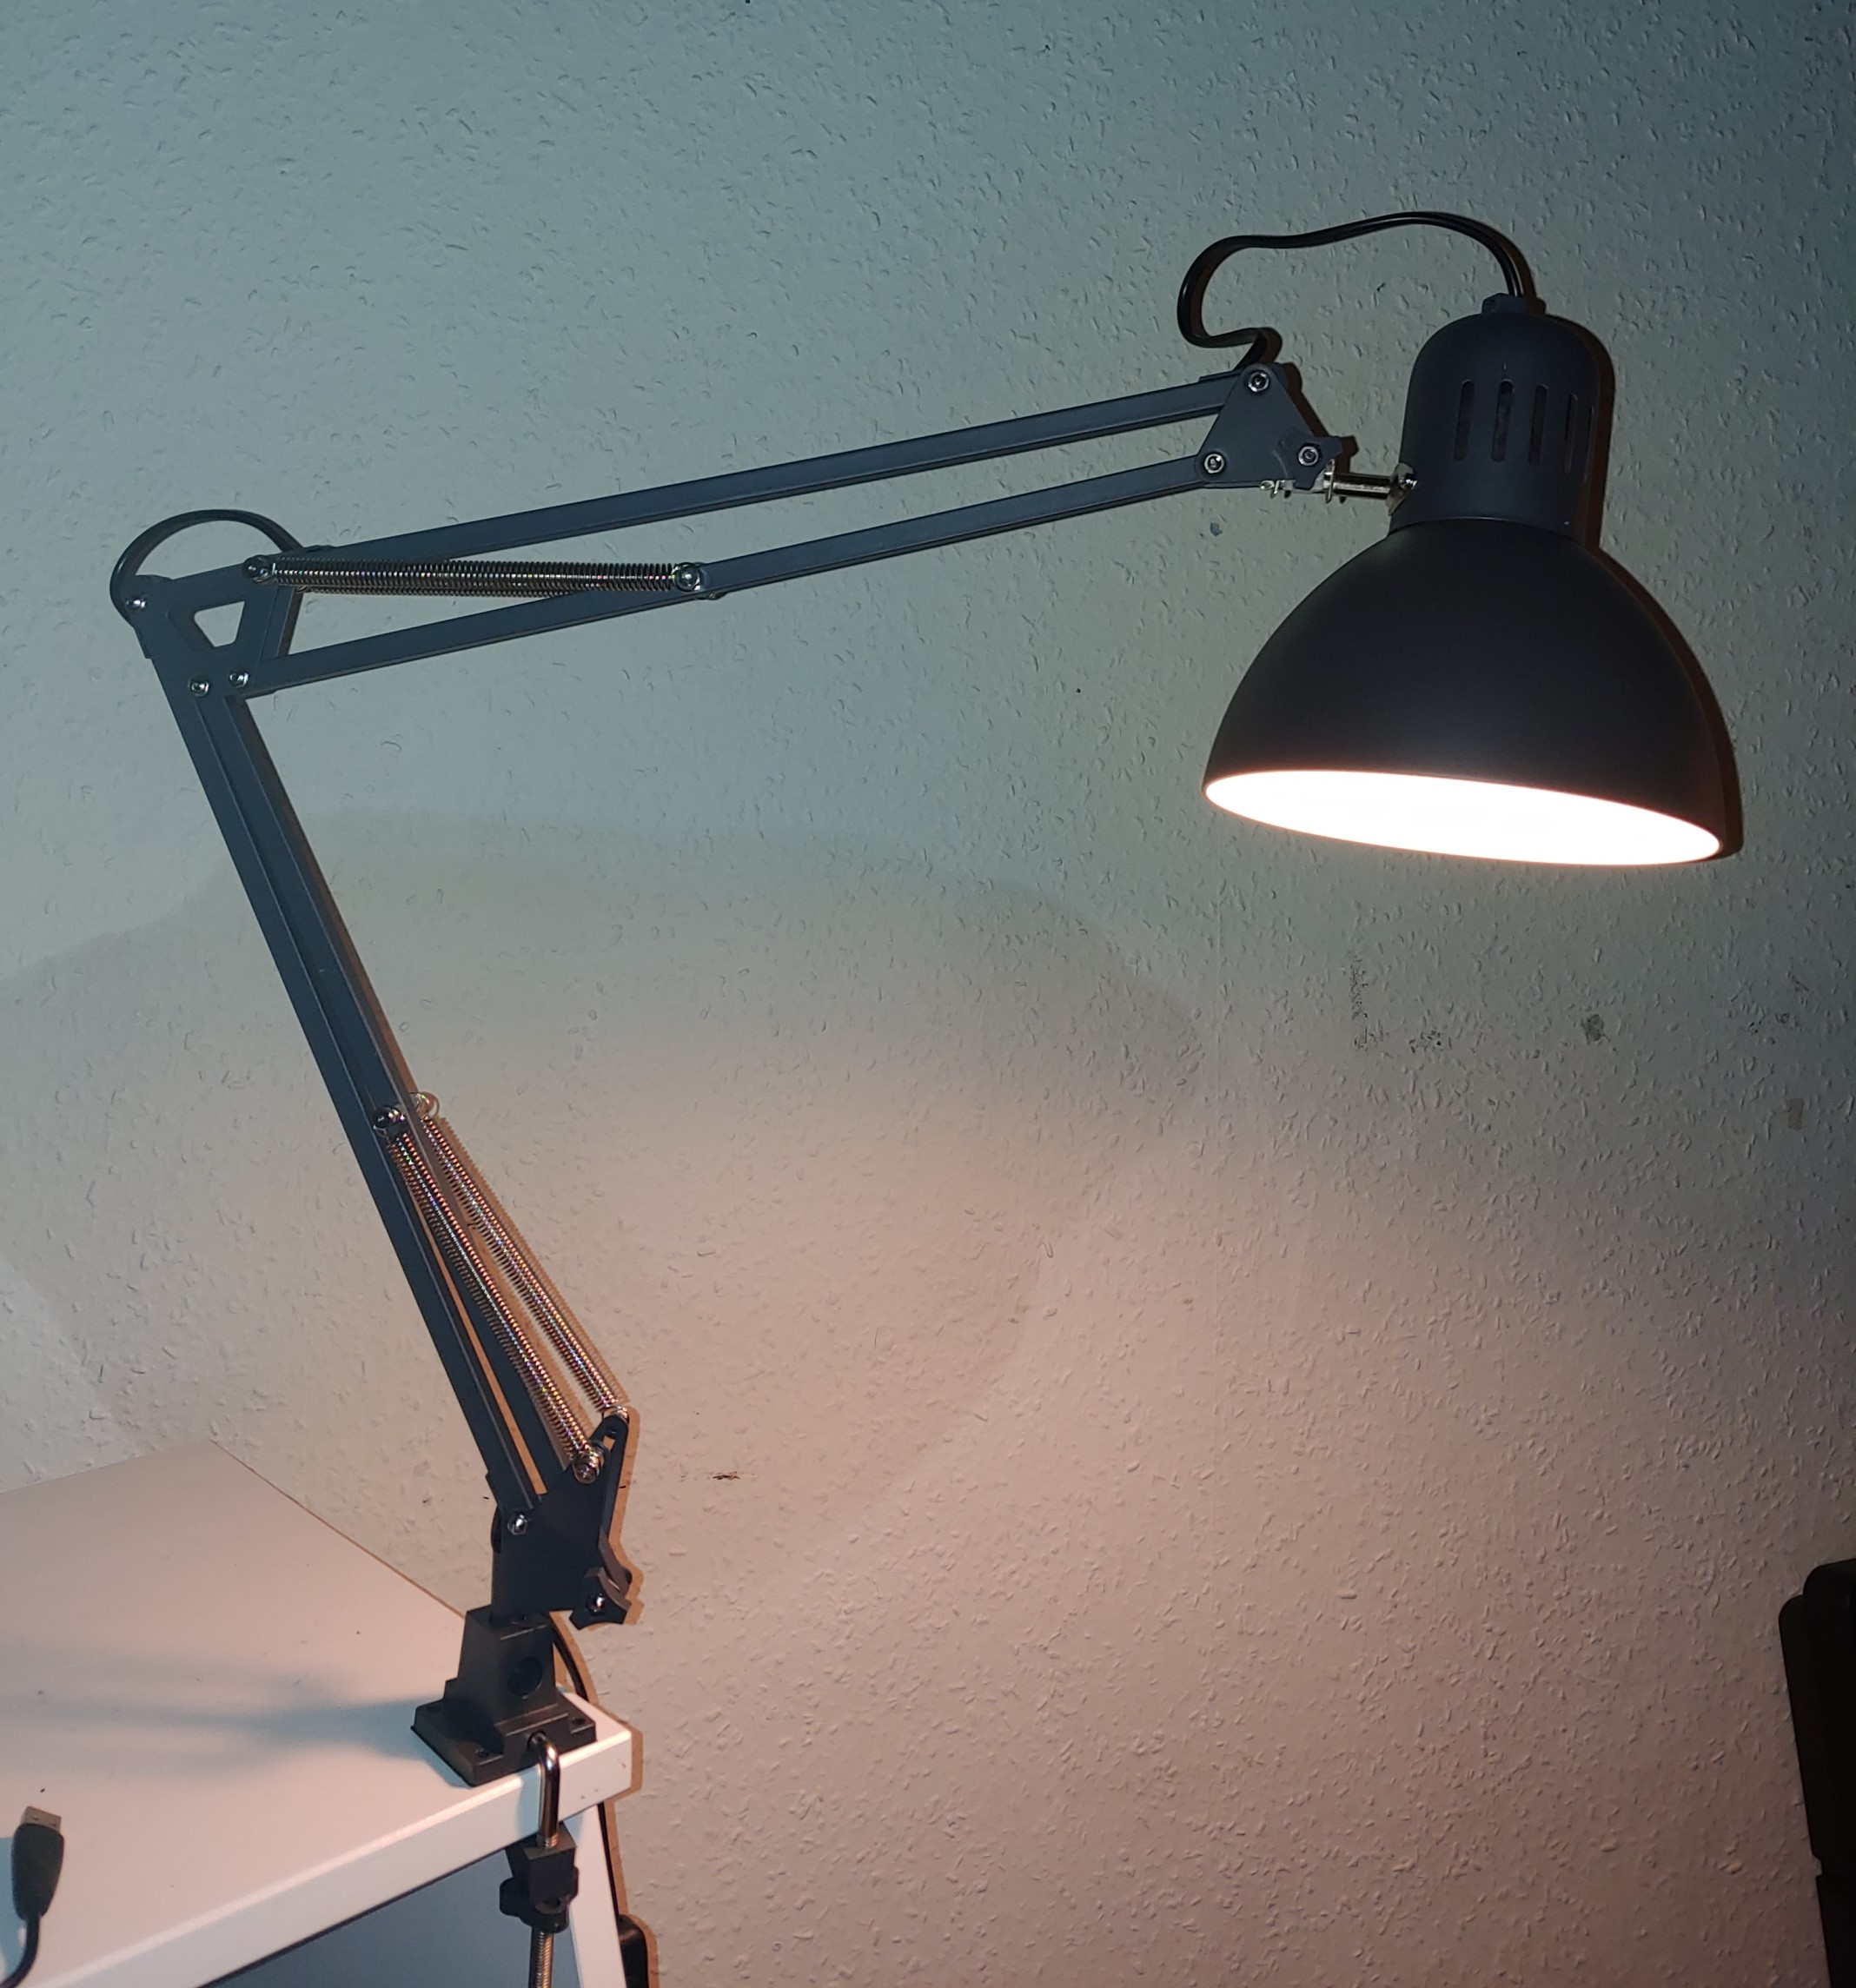
\includegraphics[width=\textwidth,height=\textheight]{Images/A1_Lamp_Picture_Rotated.jpg}
    \caption{Desk lamp}
    \end{subfigure}
    \hfill
    \begin{subfigure}[b]{0.45\textwidth}
    \centering
    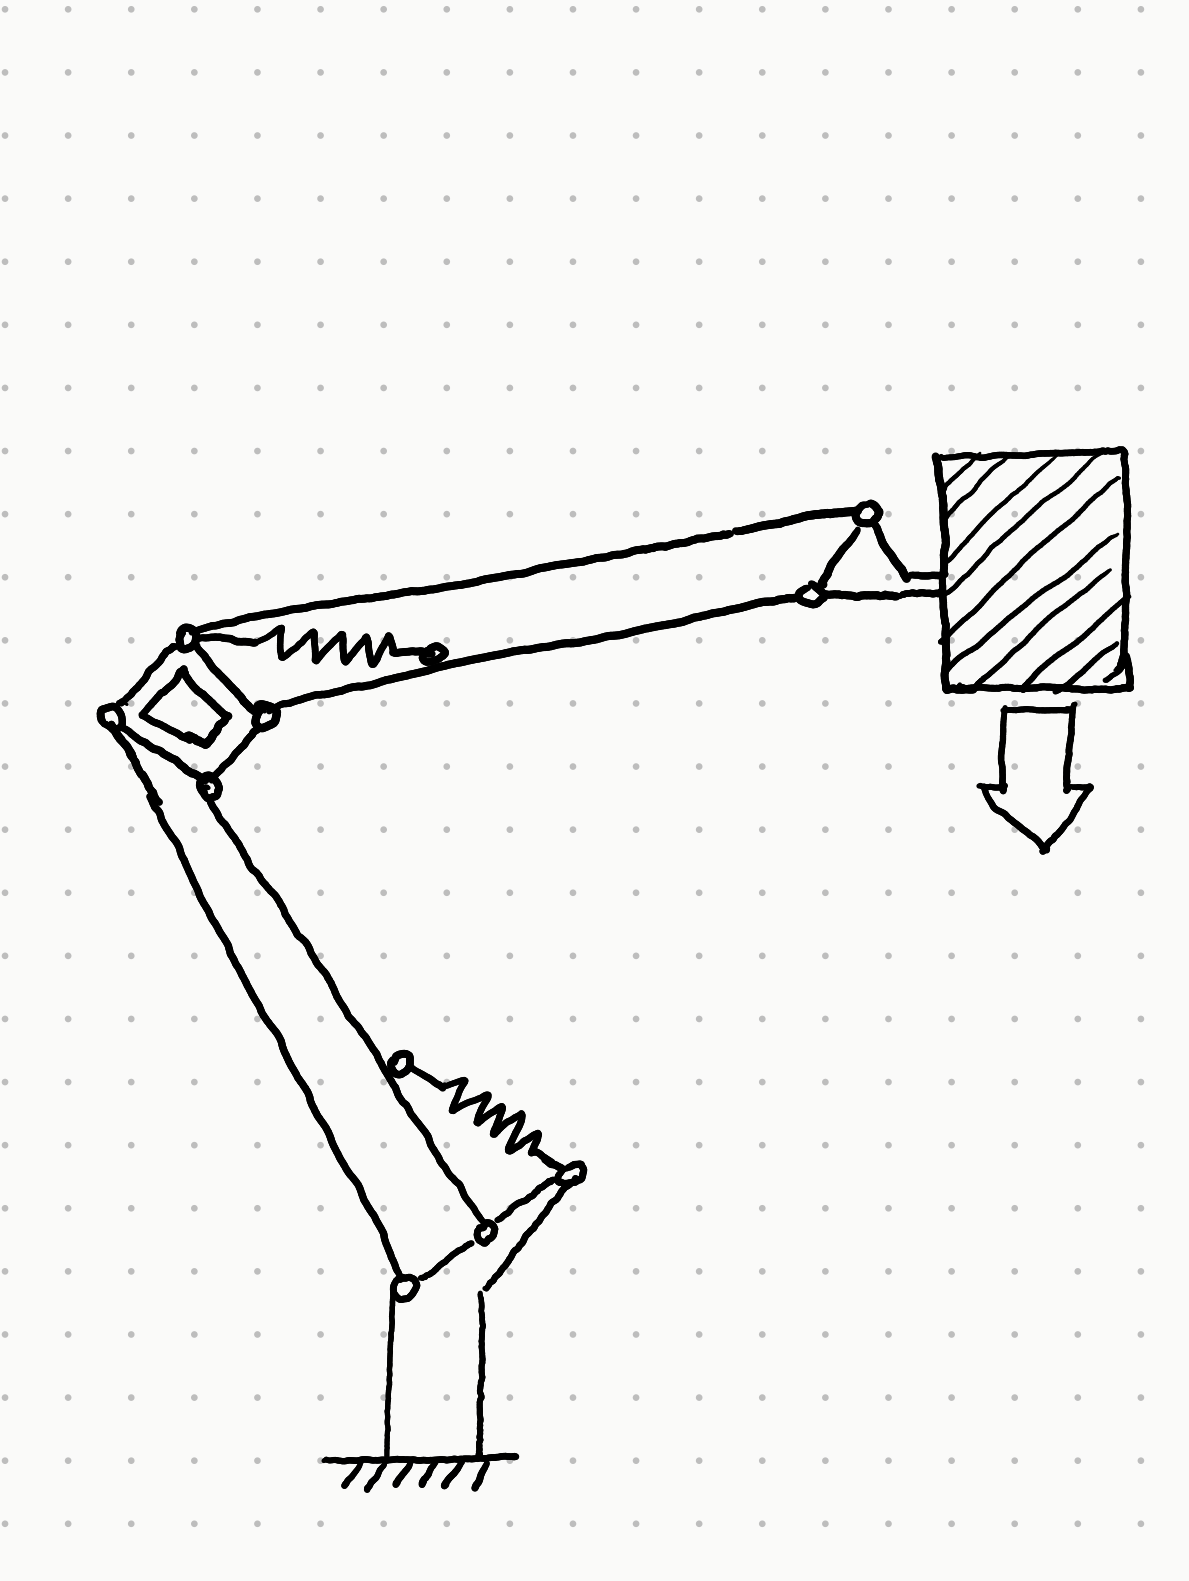
\includegraphics[width=\textwidth,height=\textheight]{Images/A1_Lamp_Diagram.png}
    \caption{Diagram of Desk Lamp}
    \end{subfigure}
\end{figure}

The lamp is represented from the side to give the best view of the
armatures. The only joint which is not represented in this view is the
connection between the body and the head of the lamp, which is a
universal joint held in place by friction. Since it's held in place by
friction rather than a balance of forces in beams or trusses, this joint
does not fit naturally into a structural diagram, and so its omission is
acceptable.

The base of the lamp is represented as a fixed support, since the lamp
is clamped to the table. The bottom part of the lamp is represented as a
beam, since it must withstand both axial and bending moments. Every
joint in the diagram represents an actual pinned joint which can rotate.
The arms of the lamp are represented as struts; since they pinned on
both ends, it is not possible for them to transmit bending forces. (This
is not strictly true for the struts with the springs attached in the
middle; one could defensibly have drawn those as beams since the springs
create a slight bending moment in those supports). The springs are drawn
as springs but could just as easily have been drawn as struts, since
they carry only axial loads.

Drawing the diagram gives a good idea of how the lamp retains its form throughout the range of motion. The pinned struts keep each section parallel (they form a parallelogram with the beam-like structures at either end), and the springs (along with some friction in the pinned joints) retain the shape of the structure through its motion.

\end{document}
